%!TEX root = ./main.tex
%
% This file is part of the i10 thesis template developed and used by the
% Media Computing Group at RWTH Aachen University.
% The current version of this template can be obtained at
% <http://www.media.informatik.rwth-aachen.de/karrer.html>.
\chapter{Hardware Prototype and Software Development}
\label{Hardware Prototype and Software Development} 
Then we proceed with showing several iterations of the hardware prototypes using pinstripe material. Furthermore we describe the disadvantages and improvements of each iteration leading to the final prototype. The software implementation is described afterwards.

\section{System Design}
\mnote{MSP430 for first prototype}
\todo{exact specification of pinstripe and micro-controller und den gripper probe Klemmkabeln!!}
All prototypes presented here are using pinstripe, a fabric with separated conductive lines. For the first prototype we were using the Texas Instruments MSP430G2452 micro-controller. Each row and column of the pinstripe has to be connected to a \emph{digitalRead} pin of the micro-controller. The MSP430 controller has 16 of these pins but only 14 can be used since two pins are used for serial communication. This results in a matrix resolution of 7 by 7 at maximum. 
\medskip
\myDefBox{Resolution in pinstripe context}{When speaking of a certain resolution of our prototype, we talk about the number of connected rows and columns. Since the pinstripe fabric is of a static size, the higher the resolution the larger the prototype gets. }

We are using the TI EK-TM4C1294XL for the advanced prototypes. This board has the ability to connect more than 40 pins for \emph{digitalRead} to operate a 20 by 20 pinstripe matrix. The board is connected to a Computer via USB for serial communication.\\

\mnote{Programming Environment: Energia IDE and Processing to gather, send and process input data}
For programming the micro-controller we are using the \href{http://energia.nu}{Energia IDE}\footnote{http://energia.nu}. It is an easy to use IDE to upload programs to the TI micro-controller. The micro-controller itself is solely responsible for sending the data of the sensor to the computer via serial communication. Meaning that it tests a pin against ground for each other line and column. A \emph{1} is written to the serial-port when it is connected to another line or column and \emph{0} otherwise. This is done for each pin where \emph{numberOfPintripes} is the number of all lines and columns. For each prototype an integer array is declared and can easily be commented and uncommented depending on the prototype. The where the pin numbers are sorted such that the first pins correspond to the x-axis and the last pins to the negative y-axis. After all pins were tested we send a line-break to determine the end of the current input.\\  \\

We are using \href{http://processing.org}{Processing}\footnote{http://processing.org}, a Java based IDE, to structure the input stream from the micro-controller for further analyses. This includes several programs which either displays the raw touch points for debugging purpose or filters and interprets the sensor data. The changes of software are described along with each hardware iteration. 

\section{Early Testing}
\mnote{better note something here}
After deciding to go for the resistive approach, the essential challenge is to find a spacing material with certain characteristics. The material should
\begin{itemize}
\item be flexible by means of being wearable.
\item reliably separate the pinstripe fabric while no touch is intended.
\item concede rather easily when intended force is applied.
\end{itemize}
We start by trying some leftovers from recent research projects. 
\todo{Find names of the fabrics and materials} 
Then we place the materials between the pinstripe fabric to examine different behaviors. We glued both layers of the pinstripe fabric to sheets of paper to eliminate stretching and curling of the fabric. Some of the the materials are cut with a laser cutter. We cut equidistant circular holes to provide space for the pinstripe layers to connect. We attached 4 by 4 pinstripes to the MSP430 micro-controller. For displaying where a touch is present, we created a simple program with Processing.
\todo{insert picture here}
\mnote{Combine materials to improve results}Almost all available materials are not well suited for our purpose, since they are either too thick, thin or stiff. When combining up to two materials, which are leading to permanent contacts on their own, the results are improving. Nonetheless it is still susceptible to the slightest bend and therefore not well suited. Therefore we are using foam for the latest prototype. 

\section{The Prototype}
In this section we will first talk about the materials and fabrics we use for our prototype and describe how it is built.

\subsection{Material}
\mnote{3 mm foam as spacing material}
After numerous trials we gathered some knowledge about the key elements needed for this technique to work properly. The first and crucial aspect is the spacing material. The prototype uses a 3 mm thick layer of foam which is coated with thin layer of cotton. Foam has the properties we need to separate the pinstripe layer while no force is applied and yield rather easily when the user presses on it. Another positive feature is the increased resistance to unintended pressure caused by bending or accidental contact with the sensor. When evaluating the prototype we will take a closer look to which extend we can bend the prototype and how it performs in marginal conditions.
\\
We use a \todo{model of lasercutter?} laser cutter to cut equidistant holes out of the foam to allow the pinstripe layers to connect. This procedure leaves enough foam between the holes to retain the properties we need. 
\\ \\

\mnote{Issues with flexibility and translatory movement}
 Another problem we have to address is the stretchability and the translatory movement of the fabrics. Each time the user performs a gesture the upper layer moves in the respective direction due to the friction between the operating finger and the surface. This causes the the pinstripe fabric to shift such that the conductive stripes are not aligned to the holes properly, resulting in the prototype to stop working.  When we started testing we used needles, clips, and nails to fix the materials to each other. Not only that these methods are not well suited for wearablity, also fixing the materials exclusively at the edges is not sufficient. Nonetheless the flexibility of the pinstripe fabric can cause the shift we want to eliminate. 
\\ \\
 \mnote{Vliesofix for fixating the components of the prototype}
 To deal with the issues described above we use Vliesofix. \todo{find exact product description} Vliesofix is an adhesive on paper which can be ironed on textile. The paper can be removed afterwards and another fabric can be ironed to the corresponding textile. This results in an extensive adhesive area between two fabrics. The application of Vliesofix not only resolves the translatory movement but also the curling of the pinstripe fabric.

\subsection{Construction}
We decide two to prototypes with different dimensions. The first prototype has a resolution of 14 by 14 pinstripes and the second prototype has a resolution of 20 by 20. Since the procedure of making the prototypes is similar we only describe its building procedure for the smaller one. 
\\
We start by cutting out a \todo{determine exact size of all used materials} x by x cm piece of the 3 mm foam using the laser cutter. Then we cut out two sheet of Vliesofix with the corresponding dimensions and proceed by ironing them on both sides of the foam. This has to be done carefully since the applying heat for two long can cause the foam to melt. After cooling down the foam looses the desired properties to a certain degree. When removing the iron too soon the Vliesofix might not be adhesive enough. 
\\ \\
Once the material is cooled off we can remove the paper of the Vliesofix. We proceed with cutting the holes in the foam with the Vliesofix. Making the laser cutter cut more rows and columns of holes ensures that the resistance of the foam is the same throughout the touch sensitive area. Otherwise more force is needed at the edges than the center. 
\\
To prepare the two pinstripe layer to adhere it to the foam we again use Vliesofix first for preventing the fabric from curling and easy stretching. We do so before cutting out the pinstripe to make handling the fabric easier. Note that, while using Vliesofix with the pinstripe fabric, it is even more important to apply heat for too long. When the Vliesofix becomes liquid it gets soaked into the fabric. In some cases we ascertained that for this reason the conductivity of the pinstripes gets lost in some places. This immediately renders the sensor useless. Apart from that we do not remove the paper of the Vliesofix at this point.
\\ \\
We proceed with attaching the pinstripe layers to the foam. The stripes of each layer must be perpendicular to one another. Then we iron the untreated side of the  one pinstripe fabric to the foam and after cooling off the other pinstripe to the other side.  We have to make sure that the conductive stripes and the holes in the foam are aligned properly. Now we can remove the paper from the pinstripe fabric.
\\
After that we iron a corresponding piece of polyester on the upper side of the sensor to reduce the friction between the finger and treated pinstripe layer. The last step is to connect the sensor to the micro controller. Furthermore we connect a \todo{bluetooth module?}  Bluetooth module for wireless data stream. The power source can either be a computer or an battery pack which are connected by a micro USB cable.
 
\section{The Software}

The software is divided into two parts, the code running on the micro controller and the application running on the computer. The code for the micro controller is straight forward. We define an one dimensional array for each prototype in which the pin numbers are stored such that the first half of the array denote the horizontal x-axis starting from left to right and the second half the vertical y-axis starting from top to bottom. Now we can check each pin of the array respectively if it is connected to ground. This means that the conductive stripe connected to that pin has a connection to another stripe and a \emph{1} is sent via the serial communication and a \emph{0} otherwise. \mnote{Code for TI EK-TM4C1294XL}The line break after the \emph{for} loop lets us determine if a complete input set is received.

\mnote{Receiving the data via serial communication in Processing}
In Processing we read the data from the serial communication and store it in a buffer including the time stamp.  If at least one \emph{1} per data set is read, we consider it to be a touch. Sometimes the contact of the pinstripe layer is lost while performing a gesture due to insufficient pressure or a undersized locating surface of the operating finger. Therefore we implemented a threshold in which we can read only \emph{0} without the touch phase to end. This threshold is reset anytime if a \emph{1} is read. The raw data is logged for potential analyses as shown in figure \ref{fig:rawDataExample}.
\\ \\

\begin{figure}
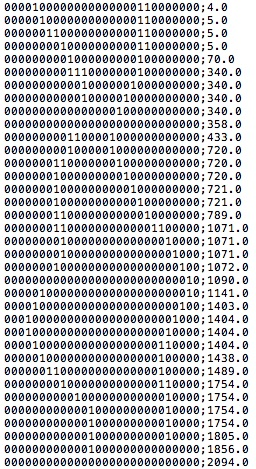
\includegraphics[scale=0.7]{images/rawDataExample.jpg}
\caption{Example of the raw data of one gesture. On the left-hand side the sensor input and on the right the time stamps in milliseconds.}
\label{fig:rawDataExample}
\end{figure}

\mnote{Use a filter algorithm to reduce the data}
Since more than one vertical and horizontal pinstripe can be connected at the same time we apply a filter algorithm. This filter algorithm takes all x-coordinates and calculates the average and the same for the y-coordinates. The resulting triple composed of the coordinate and the time stamp is added to an \emph{Arraylist} buffer. This is done for all input sets except for all those, who only consists of \emph{0's}. There are two reasons for filtering the input data. The first is the resilience to noise caused by unintended connections or slow separation of the pinstripe layers. The second reason is fact that it is easier for implementing gesture recognition. Apart from this the user intends to press only one point at the sensor.
\\
When a gesture starts we take the coordinates and subtract them from all filtered coordinates of this gesture. Therefore every gesture starts at $(0,0)$ regardless where it is performed on the sensor. This is done for the graphical representation of the strokes and will be useful later on.
\\ \\

\mnote{Implementing mark-based gesture recognition}
The next step is to actual recognize easy strokes performed on the prototype.  Since our prototypes have a rather low resolution compared to typical touch input devices we focus on rather simple unistroke gestures. These mark-based gestures are shown in figure \ref{fig:markBasedGestures}. We extend this gestures set by adding 5 gestures. These gestures are a tab and for each swipe gesture we expand it with a swipe in the opposite direction. This leads to a gesture set with 17 simple gestures. \\
 \begin{figure}
 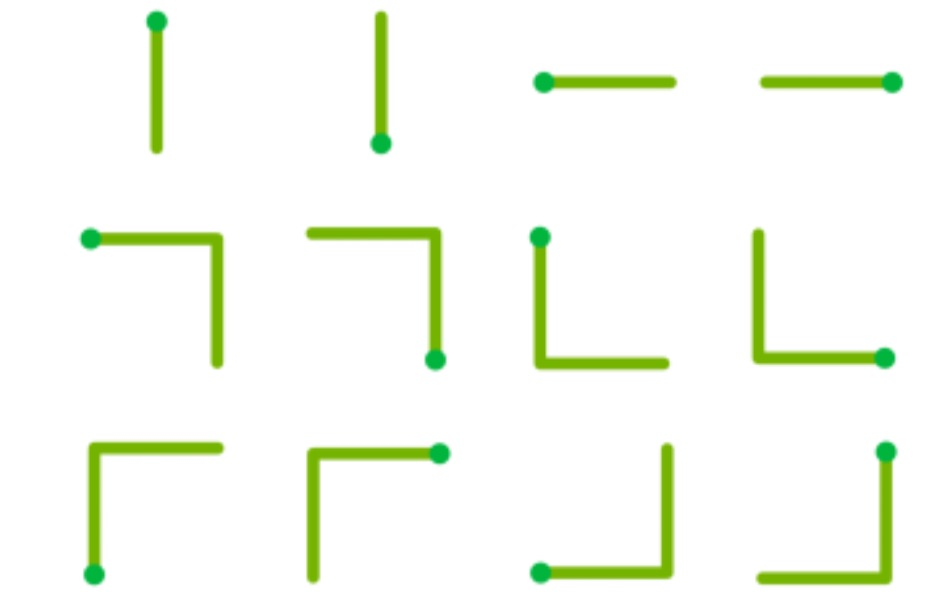
\includegraphics[scale=0.25]{images/markBasedGestures.jpg}
 \caption{Mark-based gestures. Gestures start at the dots. \cite{Bragdon}}
 \label{fig:markBasedGestures}
 \end{figure}
Our gesture recognition works as follows. First of all we do not recognize in real-time. We analyze all filtered points, stored in the buffer, after a gesture is considered finished.  Then the algorithm works as follows.
\begin{itemize}
\item check for tab
	\begin{itemize}
		\item return $true$ if the size of the buffer is $1$ 
		\item return $true$ if the all coordinates have a $distance$ smaller or equal to $1$ respectively and the time elapsed is smaller than 200 milliseconds
		\item else check for other gestures
	\end{itemize}
\item check for swipe
	\begin{itemize}
	\item assume there is a swipe with the first and the last item of the buffer as terminal points
	\item calculate the $distance$ of the line
	\item return $false$ if the $distance$ is smaller than $3$
	\item for all other points calculate the $distanceToLine$ 
	\item return $false$ if at some index the $distanceToLine$ is greater than $1$
	\item else determine the direction of the swipe and return $true$
	\end{itemize}
\item check for angle
	\begin{itemize}
	\item check if there is a line between the point at $ index - 1$ and last point in the buffer under the exact same conditions applied for swipe
	\item return $false$ if at some index the $distanceToLine$ is greater than $1$
	\item calculate the directions of both lines and return $true$
	\end{itemize}
\item end of checking 
\end{itemize}
This algorithm classifies each gesture as a tab, swipe, angle, or no gesture. In combination with the directions we calculate for each swipe we can distinguish between all 16 mark-based gestures. The orientation of a line is mapped to one of the four directions up, left, right, or down. Therefore our prototype is resilient to a certain degree of input error. With less effort we can further extend the gesture set by distinguish more directions. 
\\ \\
\mnote{Using 1\$ Unistroke Recognizer for complex gestures} 
When testing our gesture recognizer with our current prototypes we observe an almost 100\% recognition rate. Based on this finding we decide to go beyond simple mark-based gestures and continue with recognizing  more complex gestures. Therefore we make use of the 1\$ Unistroke Recognizer by \cite{Wobbrock}. This is an easy to implement recognizer which does not require any training data. Providing a template for each gesture is sufficient. A template is an array of consecutive pairs of coordinates. We can pass the coordinates in the filtered buffer straight to the 1\$ recognizer.
\\
This recognizer is orientation independent. Meaning for the marked-based gestures that, without further analysis of orientation, we can only distinguish between a swipe, an angle to the right, and an angle  to the left. However, we can recognize a set of free-form gestures shown in figure \ref{fig:freeFormGestures}.
\begin{figure}
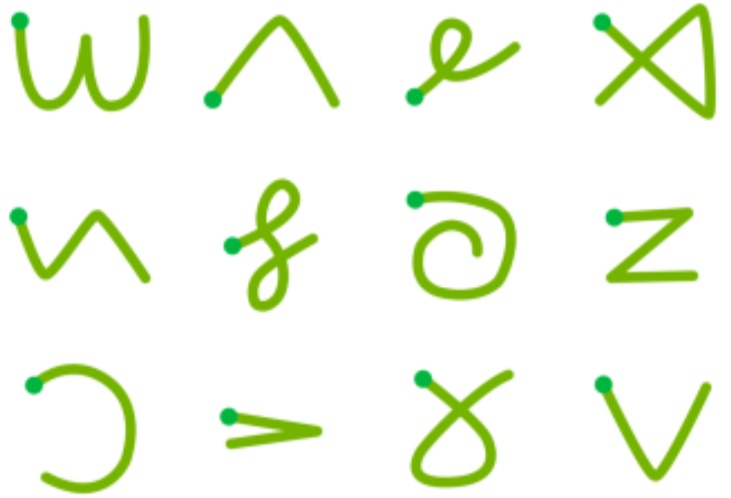
\includegraphics[scale=0.4]{images/freeFormGestures.jpg}
\caption{Free-form gestures \cite{Bragdon}}
\label{fig:freeFormGestures}
\end{figure}


\chapter{System Evaluation}
\mnote{Testing the 14 by 14 prototype}

In this chapter we will evaluate the robustness and amount of noise the system generates in different extreme conditions. We will take a closer look at the performance of the 14 by 14 prototype. Since the prototype is designed as a wearable, we are interested in its behavior under certain changing conditions. We conducted an informal user study to test the physical limitations of our prototype. 

\section{Physical Limitation Study}
\mnote{Independent variables: friction, softness, looseness, and curvature}
The human body is in motion almost all the time and the clothes we are wearing are not fixed to the skin. This \emph{looseness} and the changing subsurface are variables that may influence the performance of our prototype. Another variable is the \emph{friction} of the overlaying material. Depending on the fabric and method of fashioning, it can, more or less likely, happen that the user slips of the touch-sensing area, or experiences an unpleasant feeling in the operating finger. Furthermore the \emph{softness} of the underlying surface may influence the performance of our prototype. The human body has different softness almost everywhere. The amount of muscles, adipose tissue, and so forth also differs from human to human. This, in the first place, affects the pressure needed by the user. Then there are the different levels of curvature. Our prototype has flexible spacing-material to separate the pinstripe layer. After a certain amount of bend the material starts creasing, causing some permanent contacts. In this study we will test our prototype in conditions which aim to simulate the in field circumstances. To test to which degree of bend the prototype breaks we used different foams with the same height but different softness.

\section{Study Design}
The participants had to perform 8 different gestures in different conditions. To control the curvature, we used aerosol cans with 53 mm diameter and 66mm diameter. As a baseline we also used the table with a flat surface. When we tried to perform gestures on a curvature below 53 mm we got permanent contacts immediately. To fixate the aerosol cans we build stands using a laser cutter. The prototype was fixed with duct tape to the surface of the cans and . To achieve the curvature with the foam, we used a book and wrapped the foam around the cover and clipped it in a vise. The fabrics (jeans, cotton, \todo{brown farbric?} \todo{insert pictures}) were pinned with needles to the prototype. Nevertheless, there is still a certain amount of movement due to the flexibility of the fabrics. Since we aim to build a textile touch pad for eyes-free interaction, the user can not see the output on the screen. \\

The conditions, at least curvature and softness, were chosen at random. In order to shorten the time of the study, we tested all fabrics consecutively changing the order. Some prior testing has shown that the foam with a density of \\todo{find that paper with the numbers} xxxxxx and xxxxxxx perform alike. Thus we dropped the  foam with higher density after the first participant tested both foams in one condition without significant differences in terms of input error. \\

\todo{mention participants}The participants were filmed while interacting with the prototype. Furthermore the screen with our program was captured to determine the by eye, whether the gesture was recognized correctly or, if not, should have been recognized correctly. Additionally, our program created two log-files for every condition. One logged the filtered data and one the raw sensor data. Both files logged the time it took to perform each gesture.

\section{Study Procedure}
After the user arrived we introduced her to our prototype. We explained the basic functionality and demonstrated how the output looks like. Then we let the user test the eight gestures and some freestyle strokes. This was done without foam or any additional fabric. We pointed out that a certain amount of pressure is essential for our prototype to recognize the touch. When they felt familiar enough, about 2 minutes of testing, we prepared the first condition. 
\\ \\
For each condition we setup a GoPro Hero 3 to capture the prototype and the acting hand of the user. When we were ready to start recording the screen and setup, we told the user to continue. Since the user cannot see the output during the study, we told the user when insufficient  pressure was applied or when the touch-sensing area was left. In both cases we most likely recognized one or two wrong gestures. We represent the number of wrong gestures with an \emph{x} in the respective chart. 
\\ \\
When one condition is completed we asked the user about their impressions of the fabric, softness, and curvature. 

\section{Observation}

